% Chapter 3: Designing Experiments
\chapter{Designing Experiments}\label{chap:3}
\label{ch:designs}

This chapter explains how a new experiment is planned in REGEN: which design to choose for which goal, how each
design type is built, what the options in the \ui{New Design} dialog mean, how the \ui{Design Guide} recommends a
design and a number of runs, and how an existing design is extended with the \ui{Augment Design} dialog. The theory
is given as it is implemented in the program, so that the numbers shown by REGEN can be checked by hand.

\section{Choosing a design}
\label{sec:ch03-choosing}

A design is chosen by the question the experiment must answer, not by habit. REGEN distinguishes three main
situations.

\begin{description}[leftmargin=0pt]
\item[Screening.] Many factors (often six or more), little prior knowledge. The question is \emph{which factors
matter}. Main effects are enough; interactions and curvature can wait. Two-level fractional factorials of
resolution IV, Plackett--Burman designs and definitive screening designs answer this question with few runs
\citep{montgomery2017,jones2011}.
\item[Characterization and optimization (RSM).] Two to about six factors that are known to matter. The question is
\emph{how the response depends on them} and \emph{where the best setting lies}. Because an optimum inside the
region implies curvature, a second-order (quadratic) model is needed and every factor must have at least three
levels. Central composite, Box--Behnken and optimal (custom) designs are built for this purpose
\citep{box1951,box1960,myers2016}.
\item[Machine learning (ANN).] Strongly nonlinear responses (several bends, peaks, saturation) that a quadratic
polynomial cannot follow. An artificial neural network learns from examples, so it needs more runs and many levels
per factor, spread evenly over the whole region. Space-filling Latin hypercube designs and hybrid designs (a
classical RSM design plus space-filling points) serve this goal \citep{mckay1979,morris1995}.
\end{description}

Mixtures (the factors are proportions that add up to a fixed total) and experiments with hard-to-change factors
(split-plot) are special structures that can occur in all three situations; they have their own design types.
Table~\ref{tab:ch03-choice} summarizes the choice.

\begin{table}[htbp]
\centering
\caption{Which design type for which goal (k = number of numeric factors).}
\label{tab:ch03-choice}
\small
\begin{tabularx}{\linewidth}{@{}p{3.3cm}p{4.6cm}X@{}}
\toprule
Goal & Design types in REGEN & Typical run count (k = 3 unless stated) \\
\midrule
Screening & Fractional factorial (Res IV), Plackett--Burman, Definitive Screening, Taguchi array &
  k = 7: 16 + 4 center (2\textsuperscript{7-3}, Res IV), 12 (PB), 17 (DSD) \\
Ruggedness test & Fractional factorial (Res III), Plackett--Burman & k = 7: 8 (2\textsuperscript{7-4}), 12 (PB) \\
Main effects and interactions & Full factorial, fractional factorial Res V, optimal (2FI) & 8 + 4 center (2\textsuperscript{3}) \\
Optimization (RSM) & CCD, Box--Behnken, optimal (quadratic) & 20 (CCD), 17 (BBD), 20 (optimal) \\
Constrained region & Optimal (Custom) - Process with linear constraints & p + 5 + 5 \\
Formulation & Simplex lattice, simplex centroid, optimal mixture, combined mixture + process & 14 (lattice \{3,2\} with checks) \\
ANN modeling & Latin hypercube & 40 + 4 center (medium nonlinearity) \\
RSM and ANN together & Hybrid (CCD/BBD + space-filling) & 40 \\
Existing data & Historical data (or File $\rightarrow$ Import Data) & as available \\
\bottomrule
\end{tabularx}
\end{table}

\paragraph{Sequential experimentation.} It is usually cheaper to work in stages than to run one large design. A
typical path is: screen many factors with a resolution IV fraction or a DSD, keep the three or four important ones,
then run a factorial with center points; if the center points show curvature, add axial points to turn the
factorial into a central composite design (Section~\ref{sec:ch03-augment}). A definitive screening design can
already estimate curvature for the few active factors.

\paragraph{Example 1: screening seven factors.} A fermentation medium has seven candidate factors. The
\ui{Design Guide} (Section~\ref{sec:ch03-guide}) with goal \ui{Screening} and 7 factors proposes a Plackett--Burman
design with 12 runs (lowest power 74\,\% for a 2$\sigma$ effect), the fractional factorial
2\textsuperscript{7-3} of resolution IV with 4 center points (20 runs, lowest power 96\,\%) and a definitive
screening design with 17 runs (lowest power 91\,\%). The DSD is the best choice when curvature is suspected, the
2\textsuperscript{7-3} when two-factor interactions must at least be kept apart from main effects.

\paragraph{Example 2: optimizing an extraction.} Three factors (temperature, time, concentration) are known to
matter, and the best yield is expected inside the ranges. The goal \ui{RSM optimization} proposes a rotatable CCD
(20 runs, lowest power 72\,\%), a face-centered CCD (20 runs, 32\,\%), a Box--Behnken design (17 runs, 41\,\%) and
an optimal design with 20 runs. The built-in case study ``Extraction Optimization (Box-Behnken)'' uses the BBD;
Chapter~\ref{chap:4} compares these designs in detail.

\paragraph{Example 3: data for a neural network.} A dye adsorption process with four factors shows a pH optimum,
saturation with time and a Langmuir-type dependence on concentration. A quadratic model will not fit well. The goal
\ui{ANN modeling} with medium nonlinearity proposes a Latin hypercube with 65 runs plus 4 center points; the
minimum is 30 runs. The case study ``Dye Adsorption (ANN, 40 runs)'' contains 40 such runs.

\section{Factors, coding and conventions}
\label{sec:ch03-coding}

\paragraph{Factor letters.} Factors are named A, B, C, \dots{} in the order in which they are entered. The letter I
is skipped (it is reserved for the identity in defining relations), so the letters are
\texttt{ABCDEFGHJKLMNOPQRSTUVWXYZ} and at most 25 factors are possible. Numeric factors come first, then process
factors (combined designs), then categorical factors.

\paragraph{Coded units.} All designs are built and analyzed in coded units. A numeric (process) factor with low
limit $L$ and high limit $H$ is coded as
\begin{equation}
z = \frac{x - (L+H)/2}{(H-L)/2}, \qquad x = \frac{L+H}{2} + z\,\frac{H-L}{2},
\label{eq:ch03-coding}
\end{equation}
so the low level is $z=-1$, the high level $z=+1$ and the center $z=0$. Axial points of a rotatable CCD lie outside
this range ($|z| = \alpha > 1$).

\paragraph{Pseudo-components.} A mixture component $i$ with lower limit $L_i$ in a mixture with total $T$ is coded
as the pseudo-component \citep{cornell2002}
\begin{equation}
z_i = \frac{x_i - L_i}{T - \sum_j L_j}, \qquad x_i = L_i + z_i \Bigl(T - \sum_j L_j\Bigr),
\label{eq:ch03-pseudo}
\end{equation}
so that $\sum_i z_i = 1$ and $z_i \ge 0$. The quantity $T - \sum_j L_j$ is the \emph{span}: every component can
rise at most by the span above its lower limit. If an upper limit $U_i$ is given (optimal mixture and combined
designs), the effective upper limit is $H_i = \min(U_i, L_i + \text{span})$ and the coded upper bound is
$(H_i - L_i)/\text{span}$.

\paragraph{Categorical factors.} A categorical factor with $L$ levels is stored as the level index $0, \dots, L-1$
and enters models with effect coding: $L-1$ columns, where level $j<L-1$ has a 1 in column $j$ and the last level
has $-1$ in all columns. Blocks are coded the same way (sum-to-zero, $b$ blocks give $b-1$ columns). Most design
types cross the numeric design with every combination of categorical levels (Section~\ref{sec:ch03-categoric}).

\paragraph{Model orders.} The planned model is chosen from the orders available for the design: for process
designs \ui{Linear}, \ui{2FI (2-Factor Interaction)}, \ui{Quadratic} and \ui{Cubic} (two-level factorials and
Plackett--Burman: \ui{Linear}, \ui{2FI}, \ui{3FI}); for mixtures \ui{Linear}, \ui{Quadratic}, \ui{Special Cubic},
\ui{Cubic} (Scheff\'e models); for combined designs products such as \ui{Quadratic $\times$ Linear}. The number of
coefficients (including the intercept) of a process model with $k$ factors is
\begin{equation}
p_{\text{lin}} = 1+k,\quad p_{\text{2FI}} = 1 + k + \binom{k}{2},\quad
p_{\text{quad}} = \frac{(k+1)(k+2)}{2},\quad p_{\text{cubic}} = \binom{k+3}{3}.
\label{eq:ch03-ncoef}
\end{equation}
For $k = 3$ these are 4, 7, 10 and 20.

\section{The New Design dialog}
\label{sec:ch03-newdesign}

\paragraph{Purpose.} The \ui{New Design} dialog creates a new project with a design matrix, a randomized run order
and empty response columns.

\paragraph{How to use.}
\begin{enumerate}
\item Choose \menupath{File $\rightarrow$ New Design\dots} (Ctrl+N), the toolbar button \ui{New Design}, or
\ui{New design} on the Start Page. If the current project has unsaved changes, REGEN asks whether to save it first.
\item In the group \ui{Design Type}, select the \ui{Type:} and set the number of \ui{Numeric factors:} (the label
reads \ui{Components:} for mixtures and \ui{Factors:} for Taguchi arrays), \ui{Categorical factors:} (only for the
types that allow them) and \ui{Responses:} (1--20).
\item Set the options in the group \ui{Options}. Only the rows that apply to the selected type are shown.
\item Enter the names, units and limits of the factors in the factor table (Low and High for process factors;
Lower limit, and Upper limit where available, for mixture components), the level names of categorical factors
(separated by semicolons), and the names, units and types of the responses.
\item Read the blue information line at the bottom: it shows the number of runs and the main properties of the
design and is updated after every change.
\item Click \ui{Create Design}. The project opens on the \ui{Data} page. If you are unsure which design to use,
click \ui{Design Guide\dots}: the design chosen there fills in this dialog.
\end{enumerate}

\begin{figure}[htbp]
\centering
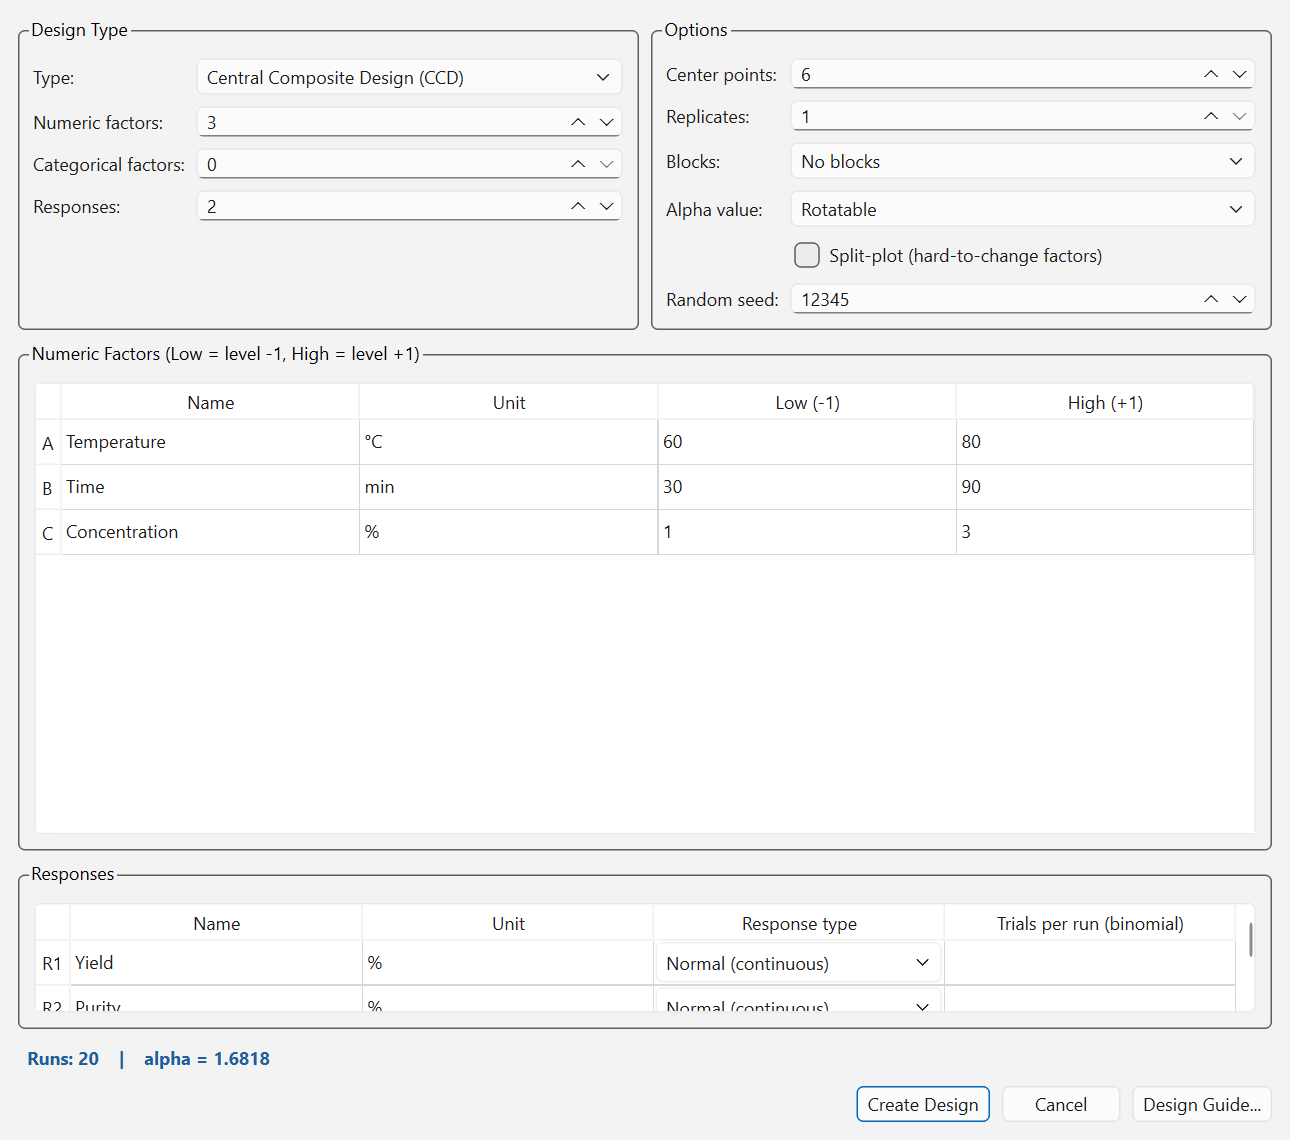
\includegraphics[width=0.75\linewidth]{new_design_ccd.png}
\caption{New Design dialog for a rotatable central composite design with three factors (Temperature 60--80
\textdegree C, Time 30--90 min, Concentration 1--3 \%), two responses and random seed 12345. The information line
reads ``Runs: 20 $|$ alpha = 1.6818''.}
\label{fig:ch03-newccd}
\end{figure}

\paragraph{Design types.} Table~\ref{tab:ch03-types} lists all types offered in the \ui{Type:} list with the
allowed number of numeric factors. The type ``Historical Data (Mixture)'' is not in the list; it is created by
\menupath{File $\rightarrow$ Import Data\dots}.

\begin{table}[htbp]
\centering
\caption{Design types of the New Design dialog.}
\label{tab:ch03-types}
\small
\begin{tabularx}{\linewidth}{@{}lcc X@{}}
\toprule
Type (as shown) & Numeric factors & Categoric & Point types created \\
\midrule
2-Level Full Factorial & 1--9 & yes & Factorial, Center \\
2-Level Fractional Factorial & 3--21 & no & Factorial, Center \\
General Factorial (Multilevel Categoric) & 0 (1--4 categoric) & required & Factorial \\
Central Composite Design (CCD) & 2--6 & yes & Factorial, Axial, Center \\
Box-Behnken Design (BBD) & 3--7 & yes & Edge, Center \\
Optimal (Custom) - Process & 1--8 & yes & Model, Lack of Fit, Replicate \\
Historical Data (Process) & 1--10 & yes & Historical \\
Screening: Plackett-Burman & 2--23 & no & Screening, Center \\
Screening: Definitive Screening Design (DSD) & 3--20 & no & Screening \\
Screening: Taguchi Orthogonal Array & 2--15 & no & Orthogonal \\
Mixture: Simplex Lattice & 3--6 & no & Vertex, Edge, Interior, Axial, Centroid \\
Mixture: Simplex Centroid & 3--6 & no & Vertex, Edge, Interior, Axial, Centroid \\
Mixture: Optimal (Custom) & 2--8 & no & Model, Lack of Fit, Replicate \\
Combined Mixture + Process (Optimal) & 2--6 comp.\ + 1--4 process & no & Model, Lack of Fit, Replicate \\
Space-filling: Latin Hypercube (for ANN) & 1--20 & yes & Space-filling, Center \\
Hybrid RSM + Space-filling (for RSM \& ANN) & 2--7 & yes & base types, Space-filling, Center \\
\bottomrule
\end{tabularx}
\end{table}

\paragraph{Options.} Table~\ref{tab:ch03-options} lists every option row of the dialog.

\begin{longtable}{@{}p{3.4cm}p{3.6cm}p{2.6cm}p{5.0cm}@{}}
\caption{Options of the New Design dialog.}\label{tab:ch03-options}\\
\toprule
Option & Values & Default & Shown for / meaning \\
\midrule
\endfirsthead
\toprule
Option & Values & Default & Shown for / meaning \\
\midrule
\endhead
\ui{Center points:} & 0--50 & CCD: 5, 6, 6, 6, 9 for k = 2--6; BBD: 5, 5, 6, 6, 6 for k = 3--7; LHS and hybrid: 4; others 0 &
  Full and fractional factorial, CCD, BBD, Plackett--Burman, LHS, hybrid. Reset when k or the type changes. \\
\ui{Replicates:} & 1--10 & 1 & Factorials, CCD, BBD, general factorial. Repeats the whole design except the center points. \\
\ui{Blocks:} & No blocks, 2, 3, 4, 8 blocks & No blocks & Only shown when blocking is possible (Section~\ref{sec:ch03-blocks}). \\
\ui{Fraction:} & ``2\textasciicircum(k-p) = N runs, Resolution R'' & smallest p & Fractional factorial. \\
\ui{Alpha value:} & Rotatable, Face-centered (alpha = 1), Orthogonal, Custom & Rotatable & CCD. \\
\ui{Custom alpha:} & 0.1--5 & 1.5 & CCD with Custom alpha. \\
\ui{Lattice degree (m):} & 1--4 & 2 & Simplex lattice. \\
\ui{Mixture total:} & 0.0001--10\textsuperscript{9} & 100 & Mixture types. \\
\ui{Add axial points + centroid} & check box & on & Simplex lattice and centroid. \\
\ui{Replicate vertices + centroid} & check box & on & Simplex lattice and centroid. \\
\ui{Criterion:} & I-optimal (best prediction), D-optimal (best coefficients) & I-optimal & Optimal types. \\
\ui{Planned model:} & orders of the design & Quadratic (combined: Quadratic $\times$ Linear) & Optimal types. \\
\ui{Additional model points:} & 0--50 & 0 & Optimal types: points chosen by the criterion beyond the p required. \\
\ui{Lack of fit points:} & 0--30 & 5 & Optimal types. \\
\ui{Replicate points:} & 0--30 & 5 & Optimal types. \\
\ui{Data rows:} & 1--5000 & 20 & Historical data: number of empty rows. \\
\ui{Plackett-Burman size:} & 12, 20, 24 runs & 12 runs & Plackett--Burman. \\
\ui{Orthogonal array:} & L4, L8, L9, L12, L16, L18, L27 & L8 (2\textasciicircum 7) & Taguchi. \\
\ui{Process factors:} & 1--4 & 1 & Combined mixture + process. \\
\ui{Split-plot (hard-to-change factors)} & check box & off & Full factorial, general factorial, CCD, BBD, optimal process. \\
\ui{Hard-to-change factors:} & factor letters, e.g.\ ``A'' or ``A, C'' & A & Split-plot. \\
\ui{Runs per whole plot:} & 0--100 (0 = automatic) & automatic & Split-plot. \\
\ui{Latin Hypercube points:} & 4--5000 & ANN target for k (k = 3: 40) & Latin hypercube; each factor gets this many levels. \\
\ui{Base design:} & CCD face-centered (3 level), CCD rotatable (5 level), Box-Behnken (3 level), Factorial (2 level) & CCD face-centered & Hybrid. \\
\ui{Space-filling points:} & 0--5000 & 12 & Hybrid. \\
\ui{Random seed:} & 1--999\,999\,999 & random number drawn when the dialog opens & All types (Section~\ref{sec:ch03-random}). \\
\bottomrule
\end{longtable}

\paragraph{Information line.} The line at the bottom of the dialog shows, depending on the type: ``Runs: N'' and
the generators of a fraction (``generator: E = ABCD, \dots''), the alpha of a CCD (``alpha = 1.6818''), the number
of blocks, the categorical crossing (``(11 $\times$ 3 categorical level combinations)''), the hard-to-change factors,
the span of a mixture (``Each component can rise up to its lower limit + 30'') or the coefficient count of an
optimal design (``Model Quadratic: 14 coefficients $\rightarrow$ 24 runs in total (14 model + 5 lack of fit + 5
replicates)''). For Latin hypercube and hybrid designs it adds a verdict on the run count for an ANN
(Section~\ref{sec:ch03-guide-calc}). A text beginning with ``Invalid:'' means the current settings cannot be built;
for example ``Invalid: PB with 12 runs allows at most 11 factors.''

\paragraph{Messages on Create Design.} Invalid inputs are reported in a message box titled ``Invalid Input'': ``The
limits of \textless name\textgreater{} are not numbers.'', ``Factor \textless name\textgreater: Low must be less
than High.'', ``The lower limit of \textless name\textgreater{} cannot be negative.'', ``The upper limit of
\textless name\textgreater{} must be greater than the lower limit.'', ``Categorical factor \textless
name\textgreater{} needs at least 2 distinct levels.'', ``The sum of the component lower limits must be less than
the total.'' and ``Response \textless i\textgreater: enter the number of trials per run ($\ge$ 1).'' (binomial
responses). Constraint errors are shown under ``Constraint'' (Section~\ref{sec:ch03-constraints}); a split-plot
without hard-to-change letters gives ``Enter the letters of the hard-to-change factors (e.g. A).''. If the
generator itself fails, the title is ``Design Could Not Be Created'', for example ``There are not enough candidate
points to estimate this model. Relax the constraints or choose a simpler model.''

\section{Two-level factorial designs}
\label{sec:ch03-factorial}

\subsection{Full factorial}
The 2\textsuperscript{k} full factorial contains every combination of the low and high levels of $k$ factors, in
standard (Yates) order with factor A changing fastest \citep{montgomery2017}. All main effects and all interactions
are estimable and orthogonal. Replicates repeat the whole set; center points are added once at the end. Center
points do not change the estimates of the factorial effects but provide pure error and a test for curvature. The
run count doubles with every factor, which limits the type to $k \le 9$ (512 runs).

\subsection{Blocking}
\label{sec:ch03-blocks}
When the runs cannot all be performed under the same conditions (several days, batches of raw material), the design
is divided into blocks and a block effect is included in the model. For a full factorial REGEN confounds selected
high-order interactions with blocks, using the generators in Table~\ref{tab:ch03-blockgen}
\citep{montgomery2017}. The block of a run is coded from the signs of the generator products,
\begin{equation}
b = \sum_{j} \Bigl[\,\textstyle\prod_{c \in w_j} z_c > 0\Bigr]\, 2^{\,j},
\label{eq:ch03-blocklabel}
\end{equation}
and the labels are renumbered in order of first appearance so that block 1 contains standard run 1. The generators
and all their products are confounded with blocks and cannot be estimated. Center points are spread evenly over the
blocks. The run order is randomized within each block, and the blocks are run in sequence.

\begin{table}[htbp]
\centering
\caption{Block generators of the 2\textsuperscript{k} full factorial.}
\label{tab:ch03-blockgen}
\small
\begin{tabular}{@{}cccc@{}}
\toprule
k & 2 blocks & 4 blocks & 8 blocks \\
\midrule
2 & AB & -- & -- \\
3 & ABC & AB, AC & -- \\
4 & ABCD & ABC, ACD & AB, BC, CD \\
5 & ABCDE & ABC, CDE & ABE, BCE, CDE \\
6 & ABCDEF & ABCF, CDEF & ABEF, ABCD, ACE \\
7 & ABCDEFG & ABCFG, CDEFG & ABC, DEF, AFG \\
\bottomrule
\end{tabular}
\end{table}

For a 2\textsuperscript{3} in two blocks with two center points, the generator ABC puts the runs with $ABC = -1$
(standard runs 1, 4, 6, 7) and one center point into block 1 and the other four runs and the second center point into
block 2. CCDs and the four-factor BBD have their own blocking rules (Sections~\ref{sec:ch03-ccd} and
\ref{sec:ch03-bbd}); other design types are not blocked when created, but augmentation can add runs as a new block.

\subsection{Fractional factorial}
\label{sec:ch03-fraction}
A 2\textsuperscript{k-p} fractional factorial uses $2^{k-p}$ runs. The first $k-p$ factors form a full factorial
(the base design); each of the $p$ added factors is set equal to the product of a group of base factors, its
\emph{generator}. For example, the 2\textsuperscript{6-2} uses E = ABC and F = BCD.

\paragraph{Defining relation.} Each generator gives a defining word $w_i = g_i \cup \{\text{new letter}\}$ (E = ABC
gives the word ABCE). The defining relation consists of the $2^p - 1$ words generated by all products of the
generator words, where letters that appear twice cancel (symmetric difference). For the 2\textsuperscript{6-2},
I = ABCE = BCDF = ADEF.

\paragraph{Word length pattern and resolution.} The word length pattern is $(A_1, A_2, \dots, A_k)$, where $A_j$
is the number of words of length $j$. The resolution is the length of the shortest word,
\begin{equation}
R = \min\{\, j : A_j > 0 \,\}.
\label{eq:ch03-resolution}
\end{equation}
In a resolution III design main effects are aliased with two-factor interactions; in resolution IV main effects are
free of two-factor interactions, but two-factor interactions are aliased with each other; in resolution V main
effects and two-factor interactions are aliased only with three-factor and higher interactions
\citep{montgomery2017}. REGEN shows the resolution in Roman numerals.

\paragraph{Aliases.} The alias of an effect $e$ with respect to the word $w$ is $e \oplus w$ (the letters in exactly
one of the two). REGEN lists the aliases of all main effects and two-factor interactions that have at most three
letters. In the 2\textsuperscript{5-2} with D = AB and E = AC (I = ABD = ACE = BCDE, word length pattern $A_3 = 2$,
$A_4 = 1$), the main effect A is aliased with BD and CE, so the design has resolution III.

\paragraph{Minimum aberration.} Different generator choices with the same resolution are not equally good. The
preferred fraction has the fewest words of the shortest length: it minimizes $A_R$, then $A_{R+1}$, and so on
\citep{fries1980}. For up to seven factors REGEN uses the textbook generators (for example 2\textsuperscript{7-3}:
E = ABC, F = BCD, G = ACD). For 8--21 factors the generators were found by computer search: maximum resolution
first, then minimum aberration; the resolution of each cell matches the standard two-level factorial table. Runs
from 4 to 512 are available.

\paragraph{Example: 2\textsuperscript{7-3}.} With generators E = ABC, F = BCD, G = ACD the defining relation has
seven words, all of length four: I = ABCE = ABFG = ACDG = ADEF = BCDF = BDEG = CEFG. The word length pattern is
$A_4 = 7$, so the resolution is IV. The main effect A is aliased only with three-factor interactions (BCE, DEF,
CDG, BFG), while AB = CE = FG. The \ui{Fraction:} list for seven factors offers 2\textsuperscript{7-1} (64 runs,
Res VII), 2\textsuperscript{7-2} (32 runs, Res IV), 2\textsuperscript{7-3} (16 runs, Res IV) and
2\textsuperscript{7-4} (8 runs, Res III).

\subsection{General factorial}
The type ``General Factorial (Multilevel Categoric)'' contains every combination of the levels of 1--4 categorical
factors (no numeric factors), repeated \ui{Replicates:} times. It is used when all factors are categorical with two
or more levels, for example three catalysts $\times$ two solvents.

\section{Screening designs}
\label{sec:ch03-screening}

\subsection{Plackett--Burman}
Plackett--Burman designs \citep{plackett1946} are two-level orthogonal arrays whose run count is a multiple of four.
REGEN builds them from the cyclic generator rows
\begin{center}\small
\begin{tabular}{@{}rl@{}}
12 runs: & \texttt{++-+++---+-}\\
20 runs: & \texttt{++--++++-+-+----++-}\\
24 runs: & \texttt{+++++-+-++--++--+-+----}
\end{tabular}
\end{center}
The design consists of the $N-1$ cyclic shifts of the generator row plus a row of all minus signs; the first $k$
columns are used ($k \le N-1$). The columns are orthogonal: $X^\top X = N I$. Main effects are partially aliased
with many two-factor interactions (each interaction is spread over several main-effect columns with coefficients
$\pm 1/3$ in the 12-run design), so these designs assume that interactions are small. Center points can be added to
detect curvature. The model is linear; the Effects plots of the analysis show main effects only.

\subsection{Definitive screening designs}
A definitive screening design \citep{jones2011} has three levels and $2m+1$ runs:
\begin{equation}
D = \begin{bmatrix} C \\ -C \\ \mathbf{0}^\top \end{bmatrix},
\label{eq:ch03-dsd}
\end{equation}
where $C$ is an $m \times m$ conference matrix: zero diagonal, $\pm 1$ elsewhere, and $C C^\top = (m-1) I$
\citep{xiao2012}. Each pair of runs $(c, -c)$ is a fold-over pair, so main effects are not aliased with any
two-factor interaction or quadratic effect, and quadratic effects are estimable. REGEN uses $m = k$ for even $k$
and $m = k+1$ for odd $k$ (the extra column is dropped), rounded up to an available order
$m \in \{4, 6, 8, 10, 12, 14, 18, 20\}$. The conference matrix is built with the Paley construction
\citep{paley1933} from the finite field with $q = m-1$ elements ($q \in \{3, 5, 7, 9, 11, 13, 17, 19\}$; GF(9) is
represented as $a + b\,i$ with $i^2 = -1 \bmod 3$): first row $(0, 1, \dots, 1)$, first column $\chi(-1)$ and
$C_{ij} = \chi(e_j - e_i)$, with $\chi$ the quadratic character of the field. The design contains one center run;
there is no option for more. Table~\ref{tab:ch03-dsd} lists the run counts. Because no Paley matrix of order 16 is
available, 15 and 16 factors use the order-18 matrix (37 runs).

\begin{table}[htbp]
\centering
\caption{Runs of the definitive screening design.}
\label{tab:ch03-dsd}
\small
\begin{tabular}{@{}lcccccccccc@{}}
\toprule
k & 3--4 & 5--6 & 7--8 & 9--10 & 11--12 & 13--14 & 15--18 & 19--20 \\
Runs & 9 & 13 & 17 & 21 & 25 & 29 & 37 & 41 \\
\bottomrule
\end{tabular}
\end{table}

A DSD estimates all main effects with high precision; a full quadratic model is estimable only when few factors
turn out to be active. With three factors, 9 runs cannot support the 10 coefficients of a full quadratic model:
Design Evaluation then reports aliased terms and only 1 residual degree of freedom. REGEN therefore uses the
\ui{Linear} model as the default for a DSD (on the Design Evaluation and RSM Analysis pages); add
two-factor interactions or squared terms only for the few factors that turn out to be active.

\subsection{Taguchi orthogonal arrays}
The arrays L4 (2\textsuperscript{3}), L8 (2\textsuperscript{7}), L16 (2\textsuperscript{15}) consist of all
interaction columns of a 2-, 3- and 4-factor full factorial (column 1 changes slowest); L9 (3\textsuperscript{4})
and L27 (3\textsuperscript{13}) are built from linear combinations over GF(3) with levels $-1, 0, +1$; L12 is the
12-run Plackett--Burman design; L18 (2\textsuperscript{1} $\times$ 3\textsuperscript{7}) is the standard table
with a two-level first column and seven three-level columns. The first $k$ columns are used. The information line
lists the levels of each factor. The signs of some interaction columns differ from printed tables; this is only a
relabelling of the levels and does not affect orthogonality. Taguchi arrays have no center points, replicates or
blocks. They are useful for screening many factors with few runs; for the analysis REGEN uses the same regression
models as for other designs, with the \ui{Linear} model as the default (signal-to-noise ratios in the Taguchi sense
are not computed).

\section{Response surface designs}
\label{sec:ch03-rsm}

\subsection{Central composite design}
\label{sec:ch03-ccd}
The CCD \citep{box1951} combines three parts: the $n_F = 2^k$ factorial points (type ``Factorial''), $2k$ axial
points at $\pm\alpha$ on each axis (type ``Axial'') and $n_C$ center points. Replicates repeat the factorial and
axial points; the center points are added once. The axial distance $\alpha$ is set by \ui{Alpha value:}
\citep{myers2016,montgomery2017}:
\begin{align}
\text{Rotatable:}\quad & \alpha = n_F^{1/4}, \label{eq:ch03-alpharot}\\
\text{Face-centered:}\quad & \alpha = 1, \label{eq:ch03-alphaface}\\
\text{Orthogonal:}\quad & \alpha = \left[\frac{n_F\,\bigl(\sqrt{N}-\sqrt{n_F}\bigr)^2}{4}\right]^{1/4},
\quad N = n_F + 2k + n_C, \label{eq:ch03-alphaorth}
\end{align}
and \ui{Custom} uses the value in \ui{Custom alpha:}. A rotatable design has a prediction variance that depends only
on the distance from the center; its five levels per factor ($-\alpha, -1, 0, 1, \alpha$) extend beyond the
low--high range, so make sure the axial settings can be run. The face-centered design keeps all points inside the
range (three levels) but estimates the quadratic terms less precisely. The orthogonal choice makes the quadratic
coefficients uncorrelated. Table~\ref{tab:ch03-ccd} gives the values with the default number of center points.

\begin{table}[htbp]
\centering
\caption{CCD with the default center points: runs and alpha.}
\label{tab:ch03-ccd}
\small
\begin{tabular}{@{}ccccc@{}}
\toprule
k & Center points & Runs & $\alpha$ rotatable & $\alpha$ orthogonal \\
\midrule
2 & 5 & 13 & 1.4142 & 1.2671 \\
3 & 6 & 20 & 1.6818 & 1.5246 \\
4 & 6 & 30 & 2.0000 & 1.7189 \\
5 & 6 & 48 & 2.3784 & 1.8963 \\
6 & 9 & 85 & 2.8284 & 2.2087 \\
\bottomrule
\end{tabular}
\end{table}

\paragraph{Blocked CCD.} With \ui{2 blocks} the factorial points form block 1 and the axial points block 2; with
\ui{3 blocks} ($k \ge 3$) the factorial points are split into two blocks by the highest-order interaction and the
axial points form block 3. Center points are distributed over all blocks in turn. If \ui{Orthogonal} is selected
together with blocks, $\alpha$ is replaced by the value that makes the blocks orthogonal to the model
\citep{montgomery2017}:
\begin{equation}
\alpha = \sqrt{\frac{n_F\,(2k + a_0)}{2\,(n_F + f_0)}},
\label{eq:ch03-alphablock}
\end{equation}
where $f_0$ is the number of center points in the factorial blocks and $a_0$ the number in the axial block. For
$k = 3$, 3 blocks and 6 center points ($f_0 = 4$, $a_0 = 2$) this gives $\alpha = 1.6330$. With \ui{Rotatable} or
\ui{Face-centered} and blocks, $\alpha$ is not changed and the blocks are then not exactly orthogonal.

\subsection{Box--Behnken design}
\label{sec:ch03-bbd}
The Box--Behnken design \citep{box1960} is a three-level design without corner points. For $k = 3, 4, 5$ every pair
of factors is run as a $2^2$ factorial ($\pm 1$) with the other factors at 0 (12, 24, 40 runs). For $k = 6$ and
$k = 7$ balanced incomplete blocks of three factors are run as $2^3$ factorials with the remaining factors at 0
(k = 6: ABD, BCE, CDF, ADE, BEF, ACF, 48 runs; k = 7: DEF, AFG, BEG, ABD, CDG, ACE, BCF, 56 runs). These runs have
the type ``Edge''. With the default center points the totals are 17, 29, 46, 54 and 62 runs. The four-factor BBD can
be split into three orthogonal blocks: pairs (A,B) and (C,D) in block 1, (A,D) and (B,C) in block 2, (A,C) and (B,D)
in block 3. A BBD is attractive when the extreme corners are dangerous, expensive or impossible; its predictions at
the corners are less precise.

\section{Mixture designs}
\label{sec:ch03-mixture}

In a mixture experiment the response depends on the proportions of the components, not on their absolute amounts,
and the components add up to a fixed total $T$ (for example 100 \%). The factors are therefore not independent, and
the models are Scheff\'e polynomials without an intercept \citep{scheffe1958,cornell2002}: linear
$\sum \beta_i z_i$, quadratic $+\sum\beta_{ij} z_i z_j$, special cubic $+\sum\beta_{ijk} z_i z_j z_k$ and full cubic
$+\sum\delta_{ij} z_i z_j (z_i - z_j)$. Designs are built in pseudo-components (Equation~\ref{eq:ch03-pseudo}).

\paragraph{Simplex lattice.} The \{q, m\} simplex lattice contains all blends whose pseudo-components take the
values $0, 1/m, \dots, 1$ and sum to one \citep{scheffe1958}; it has $\binom{q+m-1}{m}$ points (\{3,2\}: 6 points,
\{3,3\}: 10, \{4,2\}: 10). The degree $m$ should be at least the order of the planned model.

\paragraph{Simplex centroid.} For every non-empty subset $S$ of the components the blend $z_i = 1/|S|$ ($i \in S$)
is included: $2^q - 1$ points (q = 3: 7 points) \citep{cornell2002}.

\paragraph{Check blends and replicates.} \ui{Add axial points + centroid} adds the $q$ axial check blends
\begin{equation}
z_i = \frac{q+1}{2q}, \qquad z_j = \frac{1}{2q}\ (j \ne i),
\label{eq:ch03-axialblend}
\end{equation}
(for q = 3: (2/3, 1/6, 1/6)), plus the overall centroid if it is not already in the design. These interior points
allow a test of lack of fit. \ui{Replicate vertices + centroid} repeats the $q$ pure blends and the centroid so that
pure error can be estimated. Point types are assigned by the number of non-zero components: one ``Vertex'', two
``Edge'', all equal ``Centroid'', otherwise ``Interior''; check blends are ``Axial''. The simplex lattice \{3,2\}
with both options has $6 + 3 + 1 + 3 + 1 = 14$ runs; the simplex centroid for three components also has
$7 + 3 + 3 + 1 = 14$ runs.

\paragraph{Component bounds.} Lower limits restrict the region but keep it a simplex: in pseudo-components it is the
full simplex again. Upper limits (available for \ui{Mixture: Optimal (Custom)} and the combined design) cut corners
off the simplex; the region becomes an irregular polytope, and a classical lattice no longer fits. Such constrained
mixtures, and additional linear constraints, are handled by the optimal designs of Section~\ref{sec:ch03-optimal}:
the vertices of the constrained region are computed and used as candidate points.

\begin{figure}[htbp]
\centering
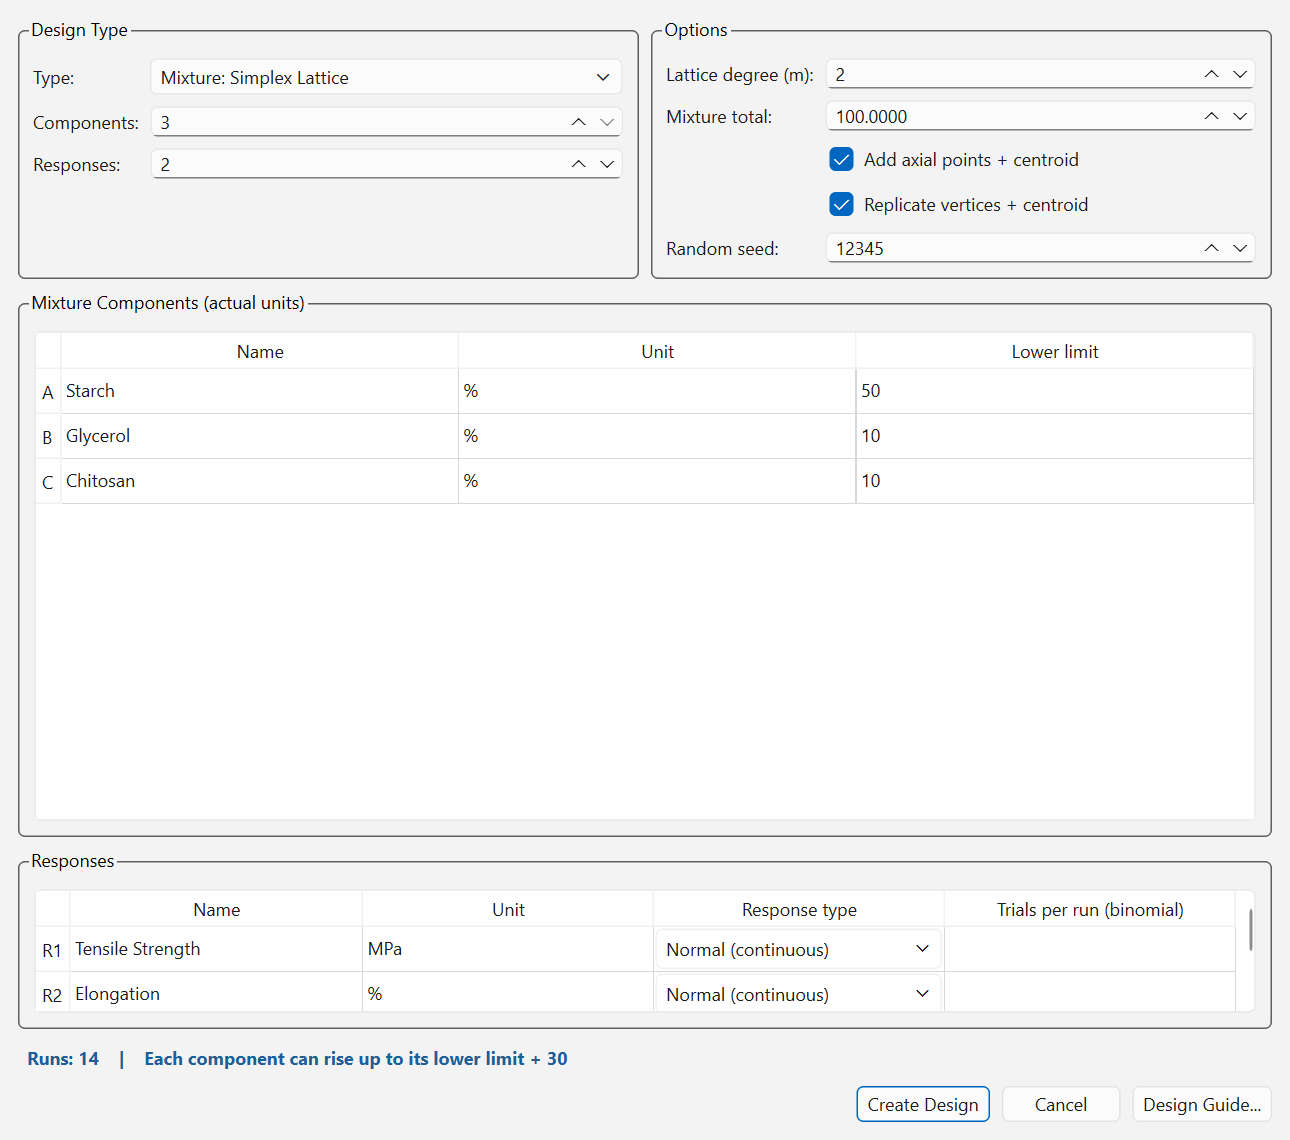
\includegraphics[width=0.75\linewidth]{new_design_mixture.png}
\caption{New Design dialog for a simplex lattice \{3,2\}: Starch (lower limit 50 \%), Glycerol (10 \%) and Chitosan
(10 \%), total 100. The information line shows 14 runs and that each component can rise up to its lower limit + 30.}
\label{fig:ch03-newmixture}
\end{figure}

\paragraph{Example: edible film.} The case study ``Edible Film Formulation (Mixture)'' (Figure~\ref{fig:ch03-newmixture})
has lower limits 50, 10 and 10 \% and total 100, so the span is $100 - 70 = 30$. The pseudo-component blend
(1/2, 1/2, 0) corresponds to Starch $50 + 0.5 \times 30 = 65$ \%, Glycerol $10 + 0.5\times 30 = 25$ \% and Chitosan
10 \%; the vertices are Starch 80 / Glycerol 40 / Chitosan 40 \%. On the Data page the check box \ui{Show
pseudo-components} switches between the two scales.

\section{Optimal (custom) designs}
\label{sec:ch03-optimal}

Optimal designs choose the runs from a set of candidate points so that a criterion is as good as possible for the
\emph{planned model} \citep{goos2011}. They are the right choice when the region is not a cube or simplex (linear
constraints, upper limits on components), when categorical and numeric factors are mixed, when the run budget does
not match a classical design, or when a mixture is combined with process factors. REGEN offers three types:
\ui{Optimal (Custom) - Process}, \ui{Mixture: Optimal (Custom)} and \ui{Combined Mixture + Process (Optimal)}.

\paragraph{Structure of the design.} An optimal design in REGEN has three parts:
\begin{itemize}
\item \emph{model points}: $n_m = p + {}$\ui{Additional model points}, chosen by the D or I criterion (type
``Model''); $p$ is the number of model coefficients, including the effect-coded columns of categorical factors;
\item \emph{lack-of-fit points}: \ui{Lack of fit points} extra distinct points, each as far as possible from the
points already chosen (type ``Lack of Fit''), so that the model can be checked;
\item \emph{replicates}: the \ui{Replicate points} distinct model points with the highest leverage are repeated
(type ``Replicate''), giving pure error.
\end{itemize}
The total is $n = p + \text{extra} + n_{\text{LOF}} + n_{\text{rep}}$. With the defaults, a two-factor quadratic
model gives $6 + 5 + 5 = 16$ runs.

\subsection{Linear constraints}
\label{sec:ch03-constraints}
For the optimal types the dialog shows the box \ui{Linear Constraints (one per line, actual units, letters =
factors/components)}. Each line is one inequality in actual units, for example
\begin{verbatim}
A + B <= 150
2A - B >= 50
\end{verbatim}
The operators \texttt{<=}, \texttt{>=}, \texttt{=<}, \texttt{=>} are accepted; \texttt{<} and \texttt{>} are
treated as $\le$ and $\ge$. Terms are written as \texttt{2A}, \texttt{2*A}, \texttt{0.5B} or \texttt{A};
constants may appear on either side; a decimal comma is accepted; letters are case-insensitive. Error messages are
``A constraint must use <= or >=.'', ``The constraint contains no factors.'', ``Factor 'X' does not exist (use
letters A--C).'' and ``Cannot read '\dots'.'', each prefixed by the line number. Constraints cannot contain
categorical factors, and in a combined design only the mixture components may appear.

Internally a constraint $a^\top x \le b$ is converted to coded units with $x = o + s \odot z$ (offset $o$ and scale
$s$ of Equation~\ref{eq:ch03-coding} or~\ref{eq:ch03-pseudo}):
\begin{equation}
G z \le h, \qquad G = a \odot s, \qquad h = b - a^\top o,
\label{eq:ch03-constraint}
\end{equation}
with $\ge$ rows multiplied by $-1$. The same constraints are respected later in region sampling (Design Evaluation,
Data Readiness) and in optimization.

\subsection{Candidate points}
The design region is the set of $z$ satisfying the bounds ($-1 \le z \le 1$ for process factors; $L \le z \le U$
with $\sum z = 1$ for mixtures) and $Gz \le h$. The candidate set contains:
\begin{enumerate}
\item the \emph{vertices} of this polytope: every combination of $d$ inequalities ($d-1$ plus the mixture equation
for mixtures) is solved as an equation system; feasible, distinct solutions are vertices;
\item \emph{edge midpoints}: the midpoint of two vertices that share at least $\dim - 1$ active constraints;
\item \emph{face centers}: the mean of the vertices on a constraint face with at least three vertices;
\item the \emph{overall centroid}, the mean of all vertices;
\item \emph{axial points} halfway between each vertex and the centroid;
\item for process factors only, the three-level grid $\{-1, 0, 1\}^d$ inside the bounds.
\end{enumerate}
Infeasible points and duplicates are removed. Process candidates are crossed with all categorical level
combinations; in a combined design each mixture candidate is crossed with the $3^{n_{\text{proc}}}$ grid of the
process factors. If the candidate matrix cannot support the model (rank $< p$), the message ``There are not enough
candidate points to estimate this model. Relax the constraints or choose a simpler model.'' appears; if the bounds
and constraints contradict each other: ``The design region is empty: the bounds and constraints contradict each
other.''

\subsection{Criteria}
Let $X$ be the model matrix of the chosen points and $M = X^\top X + 10^{-8} I$ (the small ridge keeps $M$
invertible during the search).
\begin{description}[leftmargin=0pt]
\item[D-optimal (best coefficients)] maximizes $\log\det M$. This minimizes the volume of the joint confidence
region of the coefficients; it favors points at the boundary of the region.
\item[I-optimal (best prediction)] minimizes the average prediction variance over the region,
\begin{equation}
I = \operatorname{tr}\bigl(M^{-1} W\bigr), \qquad W = \frac{1}{N_R}\, F^\top F,
\label{eq:ch03-icrit}
\end{equation}
where $F$ is the model matrix of $N_R = 3000$ points drawn uniformly from the region (uniform in the box for
process factors; for mixtures $z = L + (1 - \sum L)\,\text{Dirichlet}(1, \dots, 1)$, rejecting points above an
upper bound; points violating constraints are rejected; categorical levels at random). If fewer than 50 region
points survive, the candidate set is used instead. I-optimal designs put more points in the interior and are
recommended when the purpose is prediction and optimization \citep{goos2011}.
\end{description}

\subsection{Exchange algorithm}
The model points are found with a Fedorov-type exchange algorithm \citep{cook1980}. The search starts from $n_m$
random candidates; at each iteration every swap of a candidate $x_j$ (not yet in the design) for a design point
$x_i$ is evaluated with rank-two update formulas and the single best swap is made. With
$d_{jj} = x_j^\top M^{-1} x_j$, $d_{ii} = x_i^\top M^{-1} x_i$ and $d_{ij} = x_j^\top M^{-1} x_i$, the ratio of the
determinants after and before the swap is
\begin{equation}
\Delta_D = \frac{\det M'}{\det M} = (1 + d_{jj})(1 - d_{ii}) + d_{ij}^2 ,
\label{eq:ch03-fedorov}
\end{equation}
and the search stops when $\max \Delta_D \le 1 + 10^{-9}$. For the I criterion, with $G = M^{-1} W M^{-1}$ and
$g_{jj}, g_{ii}, g_{ij}$ defined like $d$, the reduction of $I$ follows from the Woodbury identity,
\begin{equation}
\Delta_I = \frac{(d_{ii}-1)\,g_{jj} - 2\,d_{ij}\,g_{ij} + (1+d_{jj})\,g_{ii}}{(1+d_{jj})(d_{ii}-1) - d_{ij}^2},
\label{eq:ch03-iswap}
\end{equation}
and the search stops when $\max \Delta_I \le 10^{-10}$. At most 300 iterations are made per start, from six random
starts; the best result is kept. Model points are distinct (a candidate already in the design cannot be swapped in).
Coordinate exchange \citep{meyer1995}, which works without a candidate list, is not used.

\paragraph{Lack-of-fit and replicate points.} Lack-of-fit points are added one at a time: the remaining candidate
with the largest minimum Euclidean distance to all chosen points (categorical factors one-hot encoded and divided
by $\sqrt{2}$, so that a level change counts as distance 1). Replicates are the distinct chosen points with the
highest leverage $h = x^\top (X^\top X)^{+} x$.

\paragraph{Reproducibility.} The random starts and the region sample use the \ui{Random seed:}. The same seed and
settings give the same design.

\paragraph{Example: constrained D-optimal design.} Two factors, Temperature 60--80 \textdegree C (A) and Time
30--90 min (B), with the constraints shown above, a quadratic model, D-optimal, seed 12345. The region is a pentagon
with vertices (60, 30), (60, 70), (80, 30), (80, 70) and (66.67, 83.33); the candidate set has 19 points (5
vertices, 5 edge midpoints, the centroid, 5 axial points and 3 grid points). The info line reads ``Model Quadratic:
6 coefficients $\rightarrow$ 16 runs in total (6 model + 5 lack of fit + 5 replicates)''. The six model points are
the five vertices and the centroid (69.33, 56.67); the lack-of-fit points are (70, 30), (73.33, 76.67), (60, 50),
(80, 50) and (74.67, 43.33); the five replicates repeat the five vertices. The design description is
``Optimal (Custom) - Process (D-optimal, model Quadratic) - 2 factors, 2 constraints, 16 runs''.

\begin{figure}[htbp]
\centering
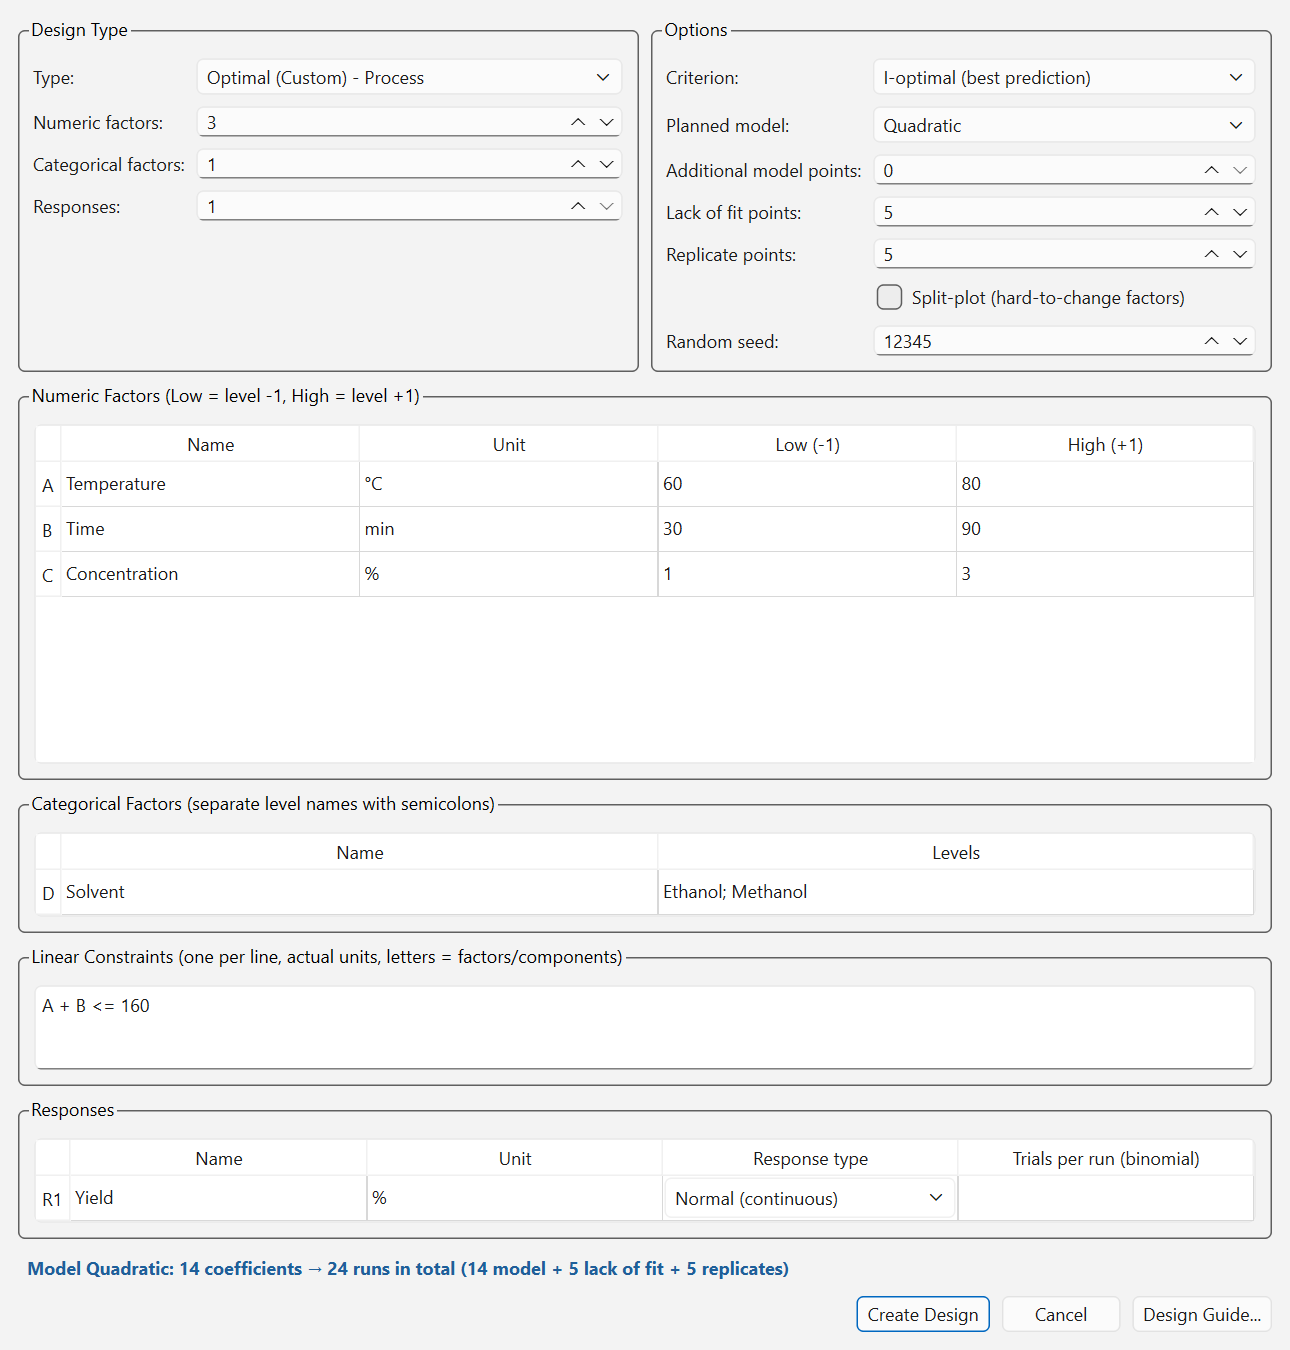
\includegraphics[width=0.75\linewidth]{new_design_optimal.png}
\caption{New Design dialog for an I-optimal process design: three numeric factors, one categorical factor Solvent
(Ethanol; Methanol), constraint \texttt{A + B <= 160}, quadratic model. Info line: ``Model Quadratic: 14
coefficients $\rightarrow$ 24 runs in total (14 model + 5 lack of fit + 5 replicates)''.}
\label{fig:ch03-newoptimal}
\end{figure}

\paragraph{I-optimal or D-optimal?} For three factors, a quadratic model and seed 12345, the ten model points of the
I-optimal design have an average prediction variance of $0.732\sigma^2$ against $0.857\sigma^2$ for the D-optimal
model points, while the D-optimal model points have the slightly larger D-efficiency (40.95 \% against 40.43 \%).
The criterion is applied to the model points only; the lack-of-fit and replicate points added afterwards change the
final values, so the complete 20-run designs can rank differently (Chapter~\ref{chap:4} compares them).

\subsection{Combined mixture and process designs}
A combined design studies $q$ mixture components and 1--4 process factors (for example a dough recipe and the
baking temperature). The model is the product of a Scheff\'e mixture model (without the cubic $\delta$ terms) and a
process model: every mixture term is multiplied by every process term. The order is written as \ui{Mixture
$\times$ Process}, for example \ui{Quadratic $\times$ Linear} (the default): the six quadratic Scheff\'e terms of
three components times (1, T) give 12 coefficients. The available orders are Linear $\times$ Mean, Linear $\times$
Linear, Linear $\times$ 2FI, Quadratic $\times$ Linear, Quadratic $\times$ 2FI, Quadratic $\times$ Quadratic,
Special Cubic $\times$ Linear and Special Cubic $\times$ 2FI. Process factors are coded $-1 \dots +1$; in the
I-optimal region sample they are uniform on $[-1, 1]$. The case study ``Cake Dough + Baking Temperature (Combined)''
(Flour 50--80, Sugar 10--30, Fat 10--30 \%, total 100; Temperature 160--200 \textdegree C) has 22 runs: 12 model, 5
lack-of-fit and 5 replicate points.

\section{Space-filling designs for neural networks}
\label{sec:ch03-spacefilling}

\subsection{Maximin Latin hypercube}
A Latin hypercube with $n$ points \citep{mckay1979} gives every factor $n$ equally spaced levels between $-1$ and
$+1$ (both bounds included), each used exactly once. Random Latin hypercubes can leave points clustered, so REGEN
rearranges the levels to spread the points as evenly as possible, using the Morris--Mitchell criterion
\citep{morris1995}
\begin{equation}
\phi_p = \sum_{i<j} d_{ij}^{-p}, \qquad p = 15,
\label{eq:ch03-phip}
\end{equation}
where $d_{ij}$ is the Euclidean distance between points $i$ and $j$ in coded units. For large $p$, minimizing
$\phi_p$ maximizes the smallest distance between points (maximin) and, among designs with the same smallest
distance, reduces the number of pairs at that distance.

\paragraph{Algorithm.} The search starts with an independent random permutation for each column and improves it by
simulated annealing: pick a random column and two runs, swap their levels, update $\phi_p$ incrementally, accept the
swap if $\phi_p$ decreases or otherwise with probability $e^{-\Delta\phi/T}$. The start temperature is
$T_0 = 0.02\,\phi_0$, it is multiplied by 0.9995 each iteration, and the number of iterations is
$\min(20000, 200n)$. For $n \le 60$ two independent starts are made and the better one kept. Above 2000 points a
plain random Latin hypercube is returned without optimization. The Latin hypercube property means that each factor
is sampled uniformly over its whole range, which reduces the variance of averages compared with random sampling
\citep{stein1987}.

\paragraph{Center points.} The default 4 center points are replicated runs at the center; they are not needed for
the space filling but give an estimate of the pure error, which the ANN diagnosis uses to recognize overfitting.

\paragraph{Example.} For three factors and seed 12345, the smallest distance between two of 20 maximin points is
0.547 coded units (a random Latin hypercube of the same size: 0.182); with 40 points it is 0.404 (random: 0.089).

\subsection{Hybrid RSM and space-filling design}
The hybrid type combines a classical RSM base design without center points (\ui{CCD face-centered (3 level)},
\ui{CCD rotatable (5 level)}, \ui{Box-Behnken (3 level)} or \ui{Factorial (2 level)}) with $e$ space-filling points
and center points. The extra points are chosen by greedy maximin: a candidate pool of a Latin hypercube with
$\max(4e, 20)$ points (2000 annealing iterations) plus 4000 uniform random points is formed, and repeatedly the
candidate whose distance to the nearest existing point (base design and the center) is largest is added. The RSM
model keeps its classical structure, while the ANN receives many more levels per factor. Example: CCD
face-centered for three factors (14 points) + 12 space-filling points + 4 center points = 30 runs. The Box-Behnken
base needs at least three factors (``Box-Behnken requires at least 3 factors.'').

\section{Split-plot designs}
\label{sec:ch03-splitplot}
When a factor is hard or expensive to change (an oven temperature, a reactor pressure), complete randomization would
require resetting it for every run. In a split-plot design the runs with the same setting of the hard-to-change
(HTC) factors are grouped into \emph{whole plots}; within a whole plot only the easy-to-change factors vary
\citep{goos2011}. Tick \ui{Split-plot (hard-to-change factors)} (available for full factorial, general factorial,
CCD, BBD and optimal process designs), type the HTC letters in \ui{Hard-to-change factors:} and set \ui{Runs per
whole plot:}.

\paragraph{Construction.} Runs with identical HTC settings form a group. A group larger than the whole-plot size is
split in standard order; the automatic size is $\lceil m/2 \rceil$ for a group of $m$ runs, so every HTC setting
appears in at least two whole plots and the whole-plot error can be estimated. The runs are randomized within each
whole plot, and the whole plots are run in random order. Blocks are not used. The Data page shows an extra column
\ui{WP}, and the design description ends with, for example, ``split-plot (HTC: A; 4 whole plots)''.

\paragraph{Analysis.} Because the whole plots are a second source of random variation, the analysis uses a mixed
model fitted by REML (Chapter~\ref{chap:5}). Whole-plot factors are tested against the whole-plot error, which has few degrees
of freedom, so their tests are less powerful than those of the subplot factors.

\paragraph{Example.} The case study ``Oven Product Hardness (Split-Plot)'' is a 2\textsuperscript{3} full
factorial with two replicates (16 runs), HTC factor A (Oven Temperature) and 4 runs per whole plot, which gives 4
whole plots (Figure~\ref{fig:ch04-datasplit} in Chapter~\ref{chap:4}). Augmentation is not available for split-plot
designs: the \ui{Augment Design\dots} button is disabled and its tooltip reads ``Augmenting split-plot designs is not
supported: the new runs would need their own whole plots. Create a new split-plot design instead.''

\section{Historical data}
\label{sec:ch03-historical}
The type \ui{Historical Data (Process)} creates \ui{Data rows:} empty rows (default 20) with point type
``Historical''. On the Data page the factor cells are then editable as well as the response cells; categorical
factors take the level name or the level number. \ui{Add Rows} and \ui{Delete Selected Rows} appear for this type.
Historical data are rarely orthogonal: check them on the Design Evaluation page (VIF, correlations, efficiencies)
and the Data Readiness page before trusting a model. Existing tables are more conveniently loaded with
\menupath{File $\rightarrow$ Import Data\dots}, which also creates historical mixture projects.

\section{Categorical factors}
\label{sec:ch03-categoric}
Categorical factors (solvent type, supplier, catalyst) are allowed in full factorials, general factorials, CCD,
BBD, optimal process designs, historical data, Latin hypercube and hybrid designs (0--4 factors). Enter the level
names separated by semicolons (commas are also accepted). Except for optimal designs, the numeric design is
repeated for every combination of categorical levels (full crossing), so the run count is multiplied by
$\prod_c L_c$; the information line shows for example ``Runs: 33 (11 $\times$ 3 categorical level combinations)''
for a two-factor CCD with three center points and three solvents (case study ``Extraction with Solvent Type
(Categoric)''). In an optimal design the categorical levels are part of the candidate set, and the exchange
algorithm decides how many runs each level receives; this is much cheaper when there are several categorical
factors.

\section{Randomization and the random seed}
\label{sec:ch03-random}
Runs must be performed in random order so that drifts in equipment, materials or operators do not bias the effects
\citep{montgomery2017}. REGEN assigns a random run order: a random permutation of all runs, or, in blocked designs,
a random permutation within each block with the blocks in sequence. The \ui{Std} column keeps the standard
(construction) order; the \ui{Run} column gives the order in which to perform the runs.

\paragraph{Random seed.} The option \ui{Random seed:} (1--999\,999\,999) initializes the random numbers used for the
run order, the whole-plot order of split-plot designs and the random parts of optimal, Latin hypercube and hybrid
designs. A new random value is drawn each time the dialog opens. The same seed with the same settings creates
exactly the same design again; note the seed (it is saved in the project and shown on the Summary page), or type a
fixed value, when the design must be reproducible, for example in a report or a course. All screenshots in this
manual use seed 12345.

\section{The Design Guide}
\label{sec:ch03-guide}

\paragraph{Purpose.} The \ui{Design Guide} answers two questions before any run is made: which design suits the
goal, and how many runs are needed for an RSM model or an ANN.

\paragraph{How to open.} \menupath{File $\rightarrow$ Design Guide\dots}, \menupath{Help $\rightarrow$ Design
Guide (RSM / ANN Run Counts)\dots}, the toolbar button \ui{Design Guide}, \ui{Design guide} on the Start Page, or
\ui{Design Guide\dots} inside the New Design dialog. The guide has three tabs. \ui{Create This Design\dots} (or a
double-click on a row or cell) closes the guide and fills the New Design dialog with the chosen type, number of
factors and options; it is available on the first two tabs.

\subsection{Recommendations by goal}
\label{sec:ch03-guide-goal}
\paragraph{Options.} \ui{Goal:} (default ``RSM optimization: find the optimum (curvature present)''),
\ui{Numeric factors:} (1--21), \ui{Max run budget:} (0 = ``no limit'') and, for the ANN goals only,
\ui{Nonlinearity:} (``Low (close to quadratic)'', ``Medium'', ``High (many peaks / sharp)''). A short explanation
of the goal appears below the options.

\paragraph{Output.} The table lists the proposed designs with \ui{Runs}, \ui{Levels per factor}, \ui{Model},
\ui{Power (2$\sigma$ signal)} and \ui{Notes}; designs above the budget are grey and marked ``over budget''. The
first suitable row is selected and explained below the table: advantages, disadvantages, the lowest power among the
model coefficients with the residual degrees of freedom, the number of coefficients of the model and an ANN verdict
for the run count (Section~\ref{sec:ch03-guide-calc}).

\paragraph{Rules.} The run counts are obtained by actually building each design. The rules per goal are:
\begin{itemize}
\item \emph{Screening}: Plackett--Burman with the smallest $N \in \{12, 20, 24\}$ larger than $k$; the fractional
factorial with the fewest runs and resolution $\ge$ IV plus 4 center points (a full factorial when no such fraction
exists); a DSD for $3 \le k \le 20$.
\item \emph{Ruggedness test} (``confirm that the factors have NO effect''): Plackett--Burman and the smallest
fraction with resolution $\ge$ III.
\item \emph{Characterization}: the smallest fraction of resolution $\ge$ V plus 4 center points; the full factorial
2\textsuperscript{k} + 4 center points when $k \le 7$ and no cheaper resolution V fraction exists; an optimal 2FI
design with $p + 5 + 5$ runs.
\item \emph{RSM optimization} and \emph{RSM and ANN}: rotatable and face-centered CCD with default center points
($2 \le k \le 6$), Box--Behnken ($3 \le k \le 7$) and an optimal quadratic design with $p + 5 + 5$ runs. For
$k \ge 6$ an extra row ``Suggestion: screen first'' proposes a DSD.
\item \emph{ANN modeling}: a Latin hypercube with the ANN target (below) plus 4 center points, and the minimum
Latin hypercube plus 3 center points.
\item \emph{ANN} and \emph{RSM and ANN}: hybrid designs on CCD face-centered, Box--Behnken ($k\ge 3$) and CCD
rotatable bases with $e = \max(\text{target} - n_{\text{base}} - 4, 6)$ space-filling points and 4 center points.
\item If the budget is below the ANN minimum, a row ``Budget of B runs is below the ANN minimum'' appears; if no
Latin hypercube fits the budget, a Latin hypercube with $B - 3$ runs + 3 center points is proposed.
\end{itemize}

\paragraph{Power.} The power column is the smallest power over all non-intercept coefficients of the model, computed
as on the Design Evaluation page (Chapter~\ref{chap:4}) with signal $\Delta = 2$, noise $\sigma = 1$ and $\alpha = 0.05$: the
probability of detecting a coefficient whose low-to-high effect equals two standard deviations. Optimal designs show
no power because they are not built in the guide. For three factors the values are: CCD rotatable 20 runs 72 \%,
CCD face-centered 20 runs 32 \%, Box--Behnken 17 runs 41 \% (the weakest terms are the interactions or the squared
terms).

\begin{figure}[htbp]
\centering
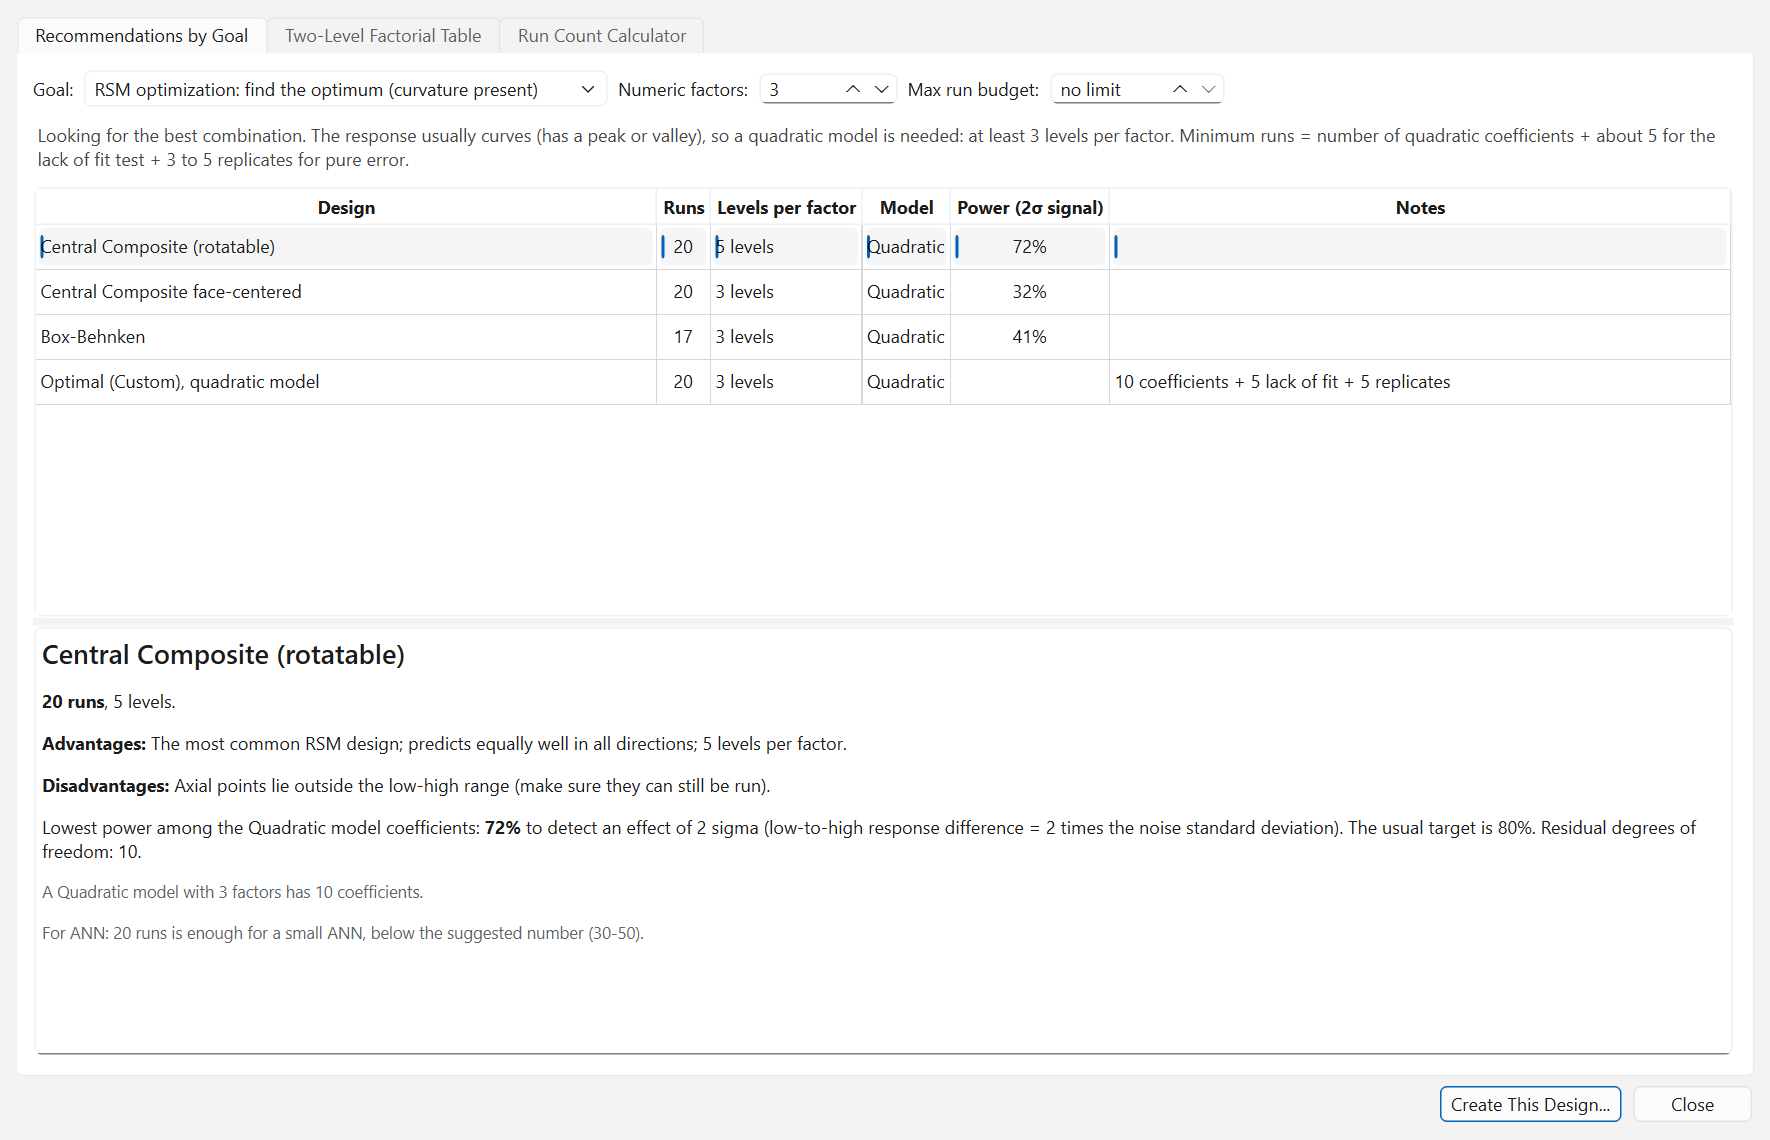
\includegraphics[width=\linewidth]{design_guide_recommend.png}
\caption{Design Guide, tab Recommendations by Goal: goal RSM optimization, 3 numeric factors. The rotatable CCD (20
runs, 5 levels, lowest power 72 \%) is selected and explained below the table.}
\label{fig:ch03-guiderec}
\end{figure}

\subsection{Two-level factorial table}
\label{sec:ch03-guide-table}
This tab shows all two-level designs for 2--21 factors (columns) and 4--512 runs (rows). Each cell gives
2\textsuperscript{k} ``full'' or 2\textsuperscript{k-p} with its resolution; the colors are white for full
factorials, green for resolution V and higher (clean main effects and two-factor interactions: characterization),
yellow for resolution IV (clean main effects: screening), red for resolution III (main effects aliased with
two-factor interactions: ruggedness testing) and grey where no design exists. \ui{Replicates:} (1--10) and
\ui{Center points:} (0--50) change the run count $N = 2^{k-p} \times \text{replicates} + \text{center points}$;
\ui{Show Generators} writes the generators into the cells of fractions with $p \le 3$.

Clicking a cell shows the design: the number of runs, the meaning of its resolution, the generators, the defining
relation (first 12 words), the word length pattern with the reminder that fewer short words mean lower aberration,
and a table of the aliases of main effects and two-factor interactions with effects of up to three letters. A note
recalls that two-level designs cannot model curvature and are not suitable for ANN or quadratic models.

\begin{figure}[htbp]
\centering
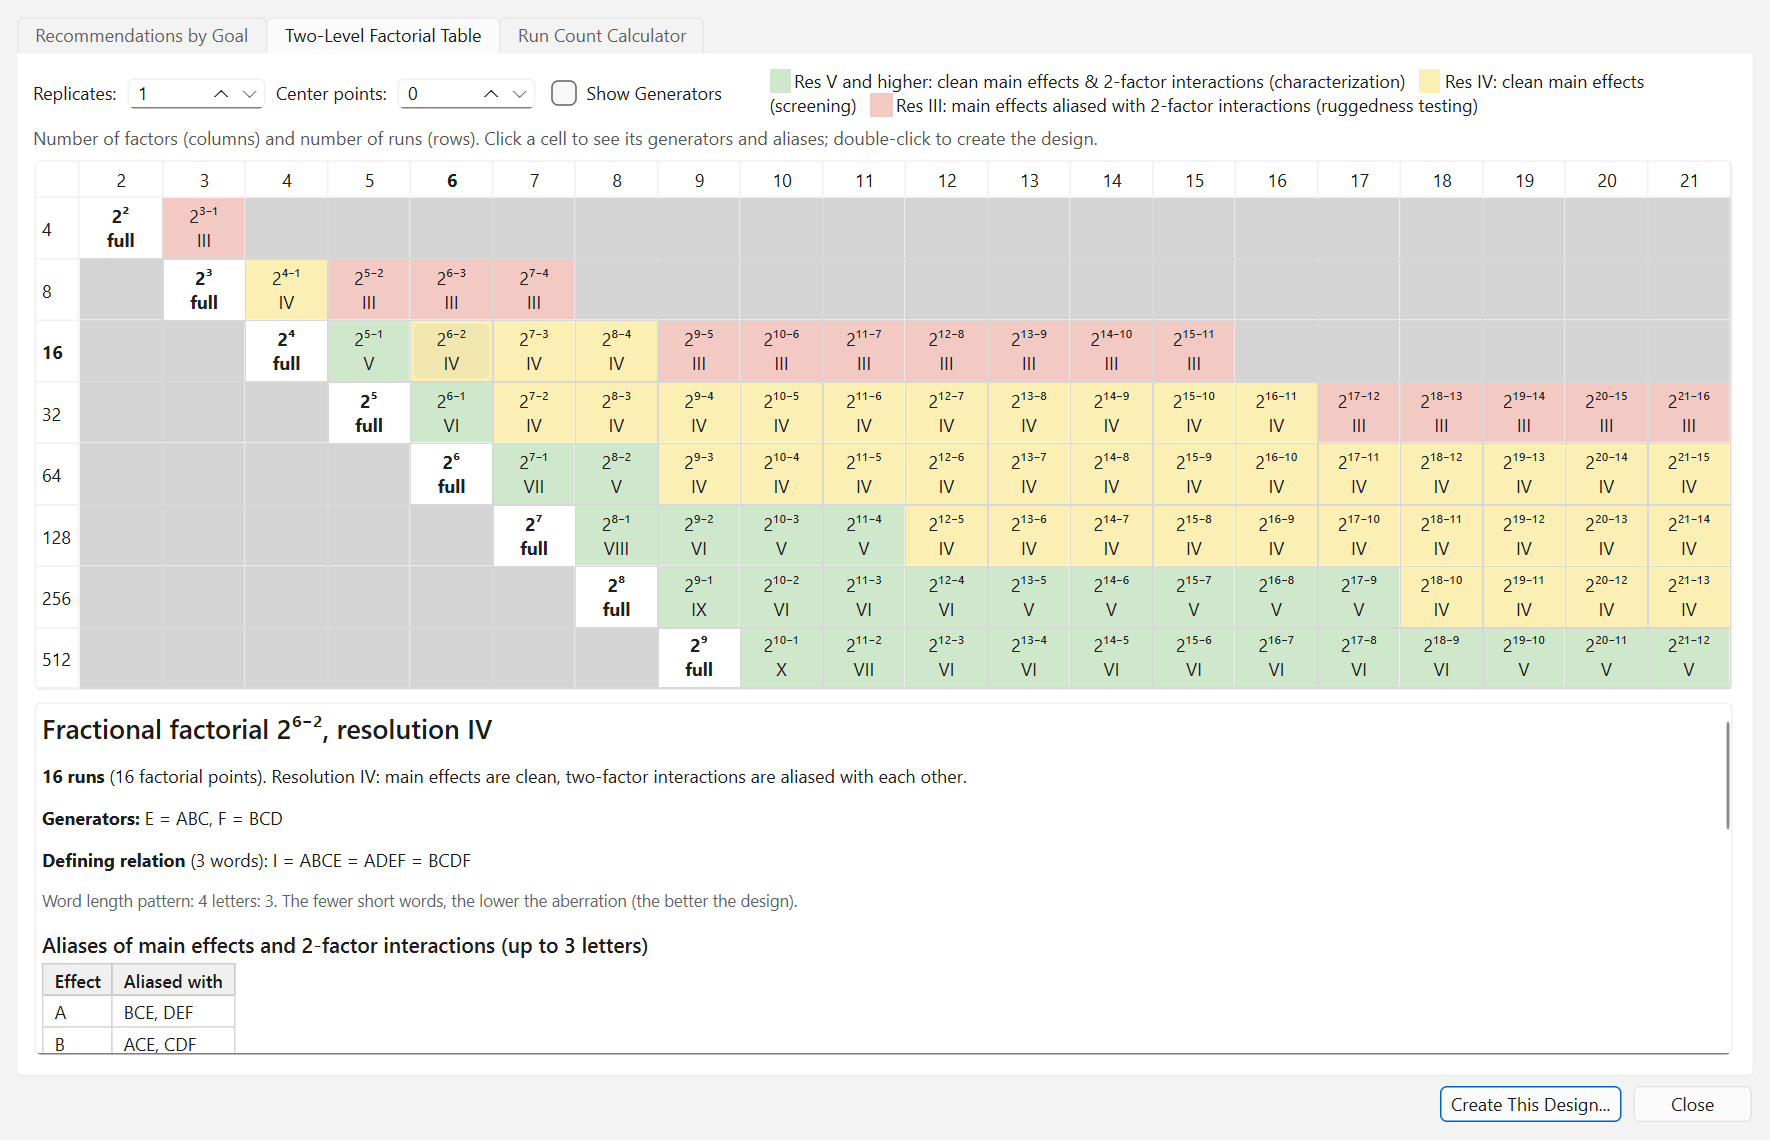
\includegraphics[width=\linewidth]{design_guide_table.png}
\caption{Design Guide, tab Two-Level Factorial Table. The selected cell (16 runs, 6 factors) is the
2\textsuperscript{6-2} of resolution IV with generators E = ABC, F = BCD, defining relation I = ABCE = ADEF = BCDF
and word length pattern ``4 letters: 3''.}
\label{fig:ch03-guidetable}
\end{figure}

\subsection{Run count calculator}
\label{sec:ch03-guide-calc}
\paragraph{RSM.} Inputs: \ui{Numeric factors:} (1--21), \ui{Model:} (Linear, 2FI, Quadratic, Cubic),
\ui{Lack of fit points:} (default 5) and \ui{Replicate points:} (default 5). With $p$ from
Equation~\ref{eq:ch03-ncoef}:
\begin{equation}
n_{\text{abs}} = p + 1, \qquad n_{\text{rec}} = p + n_{\text{LOF}} + n_{\text{rep}} .
\label{eq:ch03-rsmruns}
\end{equation}
$n_{\text{abs}}$ is the absolute minimum (one degree of freedom for the error); $n_{\text{rec}}$ is the
recommendation, which allows a lack-of-fit test and an estimate of pure error. The table ``Standard designs for k
factors'' lists the full factorial with 4 center points and the smallest suitable fraction (linear and 2FI models,
$k \le 9$), the rotatable and face-centered CCD ($2 \le k \le 6$) and the Box--Behnken design ($3 \le k \le 7$)
with their residual degrees of freedom and lowest power (``not enough df'' when there is no residual df). Below
80 \% power, add replicates or center points, or accept that small effects may go undetected.

\paragraph{ANN.} Inputs: \ui{Neurons per hidden layer:} (empty = automatic, $2k$ neurons in one layer; several
layers as a comma or semicolon separated list), \ui{Number of outputs:}, \ui{Algorithm:} (``Bayesian Regularization
(trainbr)'' or ``Levenberg-Marquardt / Adam''), \ui{Validation:} (``k-fold cross-validation (data < 400)'' or
``Hold-out 70/15/15 (large data)'') and \ui{Data you have:}. The number of weights and biases of a network with
$k$ inputs, hidden layers $h_1, \dots, h_L$ and $n_{\text{out}}$ outputs is
\begin{equation}
W = \sum_{l=1}^{L} h_l\,(h_{l-1} + 1) + n_{\text{out}}\,(h_L + 1), \qquad h_0 = k .
\label{eq:ch03-weights}
\end{equation}
The training set should contain at least $rW$ rows, with ratio $r = 1$ for trainbr (Bayesian regularization reduces
the effective number of parameters) and $r = 2$ for Levenberg--Marquardt or Adam. Because only a fraction $f$ of the
runs is used for training ($f = 0.85$ with k-fold cross-validation, $0.70$ with hold-out), the runs needed are
\begin{equation}
n_{\text{need}} = \left\lceil \frac{r\,W}{f} \right\rceil .
\label{eq:ch03-annruns}
\end{equation}
Example: three factors and 6 hidden neurons give $W = 6 \cdot 4 + 1 \cdot 7 = 31$ and, with trainbr and k-fold,
$n_{\text{need}} = \lceil 31/0.85 \rceil = 37$; with Levenberg--Marquardt and hold-out, $\lceil 62/0.70 \rceil = 89$.

\paragraph{Rules of thumb.} Table~\ref{tab:ch03-ann} gives the practical guideline used throughout REGEN for the
number of ANN runs (trainbr with cross-validation). The \emph{ANN target} used by the guide and as the default
number of Latin hypercube points is the lower recommended value for low nonlinearity, the integer mean of the
recommended range for medium nonlinearity and the larger of the upper value and the ``highly nonlinear'' value for
high nonlinearity. These numbers are a guideline, not a law: the spread of the points matters more than their
number (use at least 5 levels per factor), and the learning curve on the ANN page shows objectively whether more data
would still help.

\begin{table}[htbp]
\centering
\caption{Rule-of-thumb run counts for ANN models and the ANN target by nonlinearity.}
\label{tab:ch03-ann}
\small
\begin{tabular}{@{}ccccccc@{}}
\toprule
k & Minimum & Recommended & Highly nonlinear & Target low & Target medium & Target high \\
\midrule
1 & 10 & 15--20 & 30 & 15 & 17 & 30 \\
2 & 15 & 25--30 & 40 & 25 & 27 & 40 \\
3 & 20 & 30--50 & 60 & 30 & 40 & 60 \\
4 & 30 & 50--80 & 100 & 50 & 65 & 100 \\
5 & 40 & 70--120 & 150 & 70 & 95 & 150 \\
6 & 50 & 100--150 & 200 & 100 & 125 & 200 \\
$>6$ & $10k-10$ & $17k$--$25k$ & $35k$ & $17k$ & mean & $35k$ \\
\bottomrule
\end{tabular}
\end{table}

\paragraph{ANN verdict.} For $n$ runs and $k$ factors the verdict text (also shown in the New Design information
line for Latin hypercube and hybrid designs) is: below the minimum, ``n runs is below the practical minimum (\dots)
for k factors''; below the lower recommended value, ``enough for a small ANN, below the suggested number''; below
the highly nonlinear value, ``matches the suggested number''; otherwise ``enough for strongly nonlinear patterns''.

\paragraph{Your data.} When \ui{Data you have:} is set, the calculator states whether the data are enough for the
RSM model ($n \ge n_{\text{rec}}$) and gives the ANN verdict, adding ``This architecture needs about
$n_{\text{need}}$ runs'' when the data are fewer.

\begin{figure}[htbp]
\centering
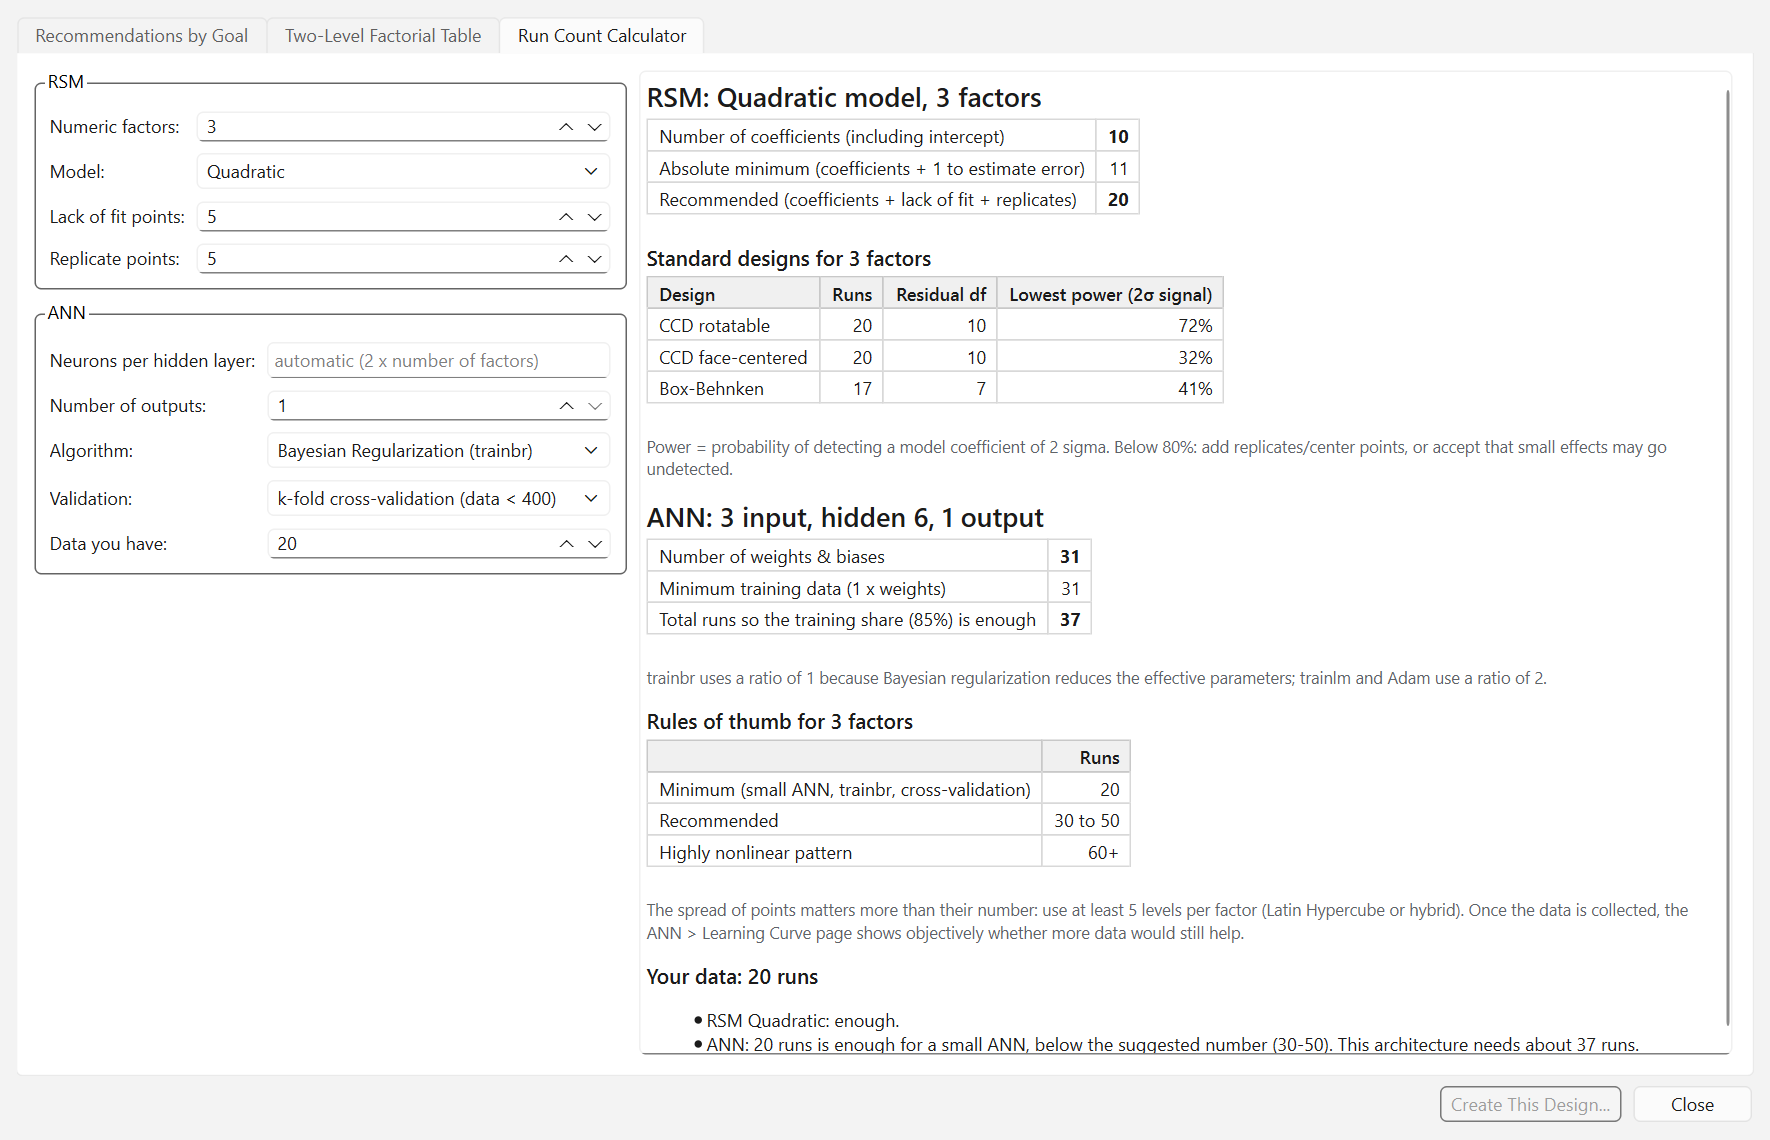
\includegraphics[width=\linewidth]{design_guide_calculator.png}
\caption{Design Guide, tab Run Count Calculator: 3 factors, quadratic model (10 coefficients, absolute minimum 11,
recommended 20 runs), standard designs with their power, and an ANN with automatic hidden size (6 neurons, 31
weights and biases) for ``Data you have'' = 20.}
\label{fig:ch03-guidecalc}
\end{figure}

\section{Augmenting a design}
\label{sec:ch03-augment}

\paragraph{Purpose.} Augmentation adds runs to an existing design without discarding the runs already made:
center points to check curvature or estimate pure error, replicates, axial points that turn a factorial into a
central composite design, or a fold-over that breaks aliases.

\paragraph{How to use.}
\begin{enumerate}
\item On the \ui{Data} page click \ui{Augment Design\dots} (not shown for historical data; disabled for
split-plot designs).
\item Choose the \ui{Type:} and set the count, alpha or fold-over factor.
\item Leave \ui{Make it a new block} checked when the new runs are made at a different time (recommended; the block
absorbs any shift between the two stages).
\item Click \ui{Add}. The message ``n new runs added. Enter their response values in the table.'' appears. The new
runs get run numbers after the current maximum, in random order among themselves, and empty responses.
\end{enumerate}

\begin{table}[htbp]
\centering
\caption{Options of the Augment Design dialog.}
\label{tab:ch03-augment}
\small
\begin{tabularx}{\linewidth}{@{}p{4.2cm}p{2.5cm}X@{}}
\toprule
Type & Available for & What is added \\
\midrule
\ui{Add center points} & all designs & \ui{Center points:} (1--50, default 3) center runs per categorical level
combination; for mixtures the overall centroid of the mixture region (type ``Centroid''). New block off by default. \\
\ui{Replicate the whole design} & all designs & \ui{Replicates:} copies of all runs with their point types. \\
\ui{Factorial $\rightarrow$ CCD (add axial + center points)} & full and fractional factorials, $\ge 2$ numeric
factors & $2k$ axial points at $\pm\alpha$ (\ui{Alpha:} Rotatable or Face-centered (alpha = 1)) plus
\ui{Additional center points:}, per categorical level combination. The design type becomes CCD. \\
\ui{Foldover (reverse signs)} & fractional factorials & A copy of all runs with all numeric signs reversed
(\ui{All factors (full foldover)}) or only one factor reversed (\ui{Only A: \dots}). Type ``Foldover''. \\
\bottomrule
\end{tabularx}
\end{table}

\paragraph{Theory as implemented.}
\begin{itemize}
\item \emph{Center points of a mixture.} The overall centroid of the (constrained) mixture region is the mean of the
vertices of the region; for a full simplex it is $(1/q, \dots, 1/q)$. Process factors of a combined design are set
to 0. For the case ``Cake Dough + Baking Temperature'' (vertices (50, 30, 20), (50, 20, 30), (80, 10, 10),
(60, 10, 30), (60, 30, 10)) the added centroid is Flour 60, Sugar 20, Fat 20 \%, whereas the mean of the existing
22 runs would be a different, unbalanced blend.
\item \emph{Factorial to CCD.} The rotatable axial distance is $\alpha = n_F^{1/4}$ with $n_F$ the number of
factorial runs of the core per categorical combination, replicates included \citep{myers2016}. A 2\textsuperscript{4}
(16 runs) gets $\alpha = 2$; a 2\textsuperscript{5-1} (16 runs) also gets $\alpha = 2$. For a fractional core the
description states it, for example ``axial points (alpha 2) on a 2\textasciicircum(5-1) fractional factorial
core''. The core must have resolution V or more for the quadratic model to be free of aliasing between
two-factor interactions.
\item \emph{Fold-over.} Reversing all signs of a resolution III fraction gives a combined design in which main
effects are no longer aliased with two-factor interactions \citep{montgomery2017}; reversing one factor frees that
factor and its two-factor interactions. For the 2\textsuperscript{7-4} (8 runs, Res III), the full fold-over gives
16 runs in which all seven main effects are orthogonal to each other and to the block (VIF 1, power 92.7 \% for
$\Delta = 2\sigma$ with the linear model).
\end{itemize}

\begin{figure}[htbp]
\centering
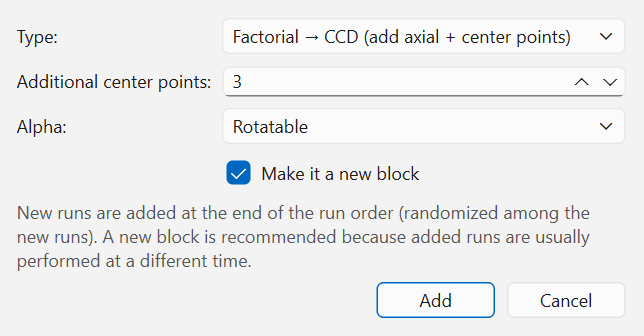
\includegraphics[width=0.6\linewidth]{augment_dialog.png}
\caption{Augment Design dialog for the 2\textsuperscript{4} factorial of the fermentation case: Factorial
$\rightarrow$ CCD with 3 additional center points, rotatable alpha, as a new block.}
\label{fig:ch03-augment}
\end{figure}

\paragraph{Example: from screening to optimization.} The case study ``Fermentation Screening (2\textasciicircum 4
Factorial)'' has 16 runs. Augmenting it with \ui{Factorial $\rightarrow$ CCD}, 3 center points and rotatable alpha
adds 8 axial points at $\pm 2$ and 3 center points in block 2. The design becomes ``Central Composite Design (CCD),
alpha = 2 + axial points (alpha 2) - 4 factors, 27 runs, 2 blocks'', which supports a quadratic model with a block
effect.

\paragraph{Other ways to add runs.} The Data Readiness page (Chapter~\ref{chap:4}) suggests runs computed from the current data
and model (D-optimal augmentation, gap filling, replicates, confirmation runs) and adds them with one click. For
historical data, rows are added with \ui{Add Rows}.
